% Created 2022-10-21 Fri 18:49
% Intended LaTeX compiler: pdflatex
\documentclass[hidelinks,11pt]{article}
\usepackage[utf8]{inputenc}
\usepackage[T1]{fontenc}
\usepackage{graphicx}
\usepackage{longtable}
\usepackage{wrapfig}
\usepackage{rotating}
\usepackage[normalem]{ulem}
\usepackage{amsmath}
\usepackage{amssymb}
\usepackage{capt-of}
\usepackage{hyperref}
\usepackage{caption}
\usepackage{subcaption} % sufigures facilities
\usepackage{float} % for H option
\usepackage{xcolor} % for the textcolor command
\usepackage[a4paper,width=150mm,top=25mm,bottom=25mm]{geometry} % fixes margins
\author{Marcelo Veloso Maciel}
\date{}
\title{Working Paper}
\hypersetup{
 pdfauthor={Marcelo Veloso Maciel},
 pdftitle={W4 Essay},
 pdfkeywords={},
 pdfsubject={},
 pdfcreator={Emacs 28.2 (Org mode 9.6)},
 pdflang={English}}
\usepackage[authordate,strict,backend=biber,
bibencoding=inputenc]{biblatex-chicago}

\addbibresource{~/Main/Org/org-roam-mvm/bib/refs.bib}
\begin{document}

\maketitle

% parencite for indirect citation, textcite for direct citation


\section{Introduction}\label{sec1}

Democracies might not elect democrats. In recent years, countries as diverse
as Hungary, Brazil, or even the USA have witnessed the election of closet or
wannabe authoritarians \parencite{luhrmann2018democracy, chiopris2021wolf}.
After being elected, such politicians typically adopt a set of
autocratization strategies that test the democratic robustness of the political
system \parencite{sorensen2021towards, bermeo2016democratic}. Their election is,
thus, a critical juncture for a polity \parencite{thelen2009institutional}. The
centrality of the electoral moment has lead a strand of the literature in
collective choice to wonder whether the success of wannabe autocrats is an
artifact of the current electoral systems \parencite{potthoff2021condorcet,
  kurrild2018trump, woon2020trump}. This paper shows that this hypothesis is not true in the case of the
Brazilian presidential election of 2018. Bolsonaro
was the Condorcet Winner, Borda Winner, and would have won under most of
the positional voting procedures. Therefore, his victory was based upon a solid
mandate \parencite{tabarrok2001president}.

Though it is debatable whether we can characterize the aforementioned
cases as instances of a broader autocratization wave
\parencite{cassani2020reversing, waldner2018unwelcome}, Bolsonaro's autocratic
credentials are unmistakable. Even a restricted democratic minimalist assessment
criteria would single out, for instance, his accusations against the integrity
of the electoral system, the attacks on the Supreme Court and the illegal
electoral maneuvers between the presidential two-rounds in 2022 as manifest
anti-democratic postures \parencite{przeworski1999minimalist,
  schmitter1994dangers}.

Despite the multiple historical contingencies that might explain his victory,
one might naturally wonder what role the electoral system has had in it. After
all, it is well-known that the outcome of collective choices is fundamentally
dependent on the voting procedure \parencite{riker1982liberalism}.
As Brazil's majority with run-off system, most electoral systems use merely the
first index of the voters' preference rankings
\parencite{grofman04_if_you_like_alter_vote} . How would he have fared
under informationally richer voting procedures, such as pairwise comparison
methods and positional voting procedures? Was he, and arguably other
democratically elected wannabe-autocrats, a product of decision procedures that
favor divisive candidates over more inclusive ones
\parencite{igersheim22_compar_votin_method}? Would the result have changed with a different set of candidates?

To answer those questions, I make use of a pre-electoral representative survey
to reconstruct the full 4-top rankings of the Brazilian population, using a
bayesian preference learning model \parencite{sorensen2019bayesmallows}.
Subsequently, I use this augmented data to simulate the electoral results under
both the Borda and Condorcet procedures, and simulate the result for all
positional procedures in 3 candidate sets. Finally, I discuss the significance
of the results and conclude by pointing out the limitations of the endeavor.

\section{Theory}\label{sec2}

It is non-trivial to trace alternative, counterfactual, political scenarios,
inasmuch the political system is a complex web of agents, situations, discourses
and institutions \parencite{bednar2018modeling, simon1991architecture,
  parsons1949structure, ostrom1997meaning}. However,
institutions stand out among those components as a locus of attention. Not only do they matter, as
\textcite{north1991institutions} argued, but they can be designed
\parencite{coleman1990rational}. Varying part(s) of the institutional matrix
gives us insight into what possible adjacent paths can or could have ensued
\parencite{north2018institutional}. Nevertheless, focusing primarily on the
institutions still leaves us facing a system of rule combinations
\parencite{ostrom1986agenda}. Sticking to ``close'' counterfactuals
\parencite{sep-possible-worlds, king2006dangers} is one way of reducing the
analysis's complexity while improving our inferences' reasonableness.

Within the subset of polyarchical systems, elections are consistently enumerated
as central to their functioning \parencite{riker1982liberalism}. No wonder ever
since the inception of the representative government, opening the black box of
the input-output process performed by voting mechanisms has emerged as a
recurrent preoccupation of politologists\parencite{rothschild2005axiom,mclean14_stran_histor_social_choic_contr}. Their centrality is composed of the realization that the result of collective decisions is inseparable from the
decision procedure being used and that such procedures differ in terms of their
consistency with normative evaluative criteria \parencite{saari2001chaotic,
  Sen_2012}. Voting procedures have, thus, a privileged position within the
institutional matrix of a polity, and my analysis will focus on their role in a
the critical moment of the Brazilian polity \parencite{kaminski1998revival,
  kaminski1999communism, tabarrok1999would}.

If the target system of interest had bestowed complexity upon us, now the theory
emerges as a new source of complexity. There are dozens, maybe hundreds, of
different voting procedures with distinct properties
\parencite{sep-voting-methods, felsenthal2018voting, felsenthal2012electoral}.
Majority rule, however, is a centerpiece of the democratic credo which underlies
contemporary polyarchical systems \parencite{dahl1989democracy}. Nevertheless,
its shortcomings are well understood, at least since the founding of the formal
study of voting procedures by Condorcet and Borda. Their responses to the
question of how can one then extend majoritarianism to more than two
alternatives constitute the foundation of the two main broad classes of decision
procedures: pairwise voting methods and positional voting methods.

Condorcet extended the majority rule to pairwise majority rule: apply
majority rule to all pairwise comparisons. One possible and, particularly
strong, condition that generalizes majoritarianism is the Condorcet criterion: a
a decision procedure is Condorcet consistent if it selects the candidate if there
is any that wins in all pairwise majority contests, the Condorcet Winner (CW)
\parencite{Felsenthal_1992}. Borda, on the other hand, devised a scoring scheme:
if there are say 3 alternatives \(\{A,B,C\}\) and an agent \(i\) has ranking
\(B>C>A\) then the Borda score in \(i\)'s ranking for each alternative is
\(A:B:C = 0:2:1\)\footnote{Alternatively, it can be coded as \(1:3:2\), or any
  scoring in which the difference between pair of subsequent scores is constant
  throughout the scoring vector \parencite{saari2012geometry} .}. The Borda
score for the whole profile, all voters rankings, is the sum of each alternative
score at each voter ranking. The Borda Winner (BW) is the alternative with
highest score. Underlying this scoring system, there is also a latent
generalization of majority rule: the Borda score is equivalent to summing over
the pairwise votes the alternative gets in a pairwise tournament
\parencite{nurmi2002voting}.

The notion of a mandate of a candidate lets us situate both methods vis-à-vis
the one-choice informational environment typical of large-scale majoritarian
elections. At a minimum, a candidate has a ``mandate'' as long as it has won
under the voting procedure. A candidate has more mandate, however, the more significant
the difference between its vote share or score vs. the second most well-voted
candidate. Note that being a CW is an even more robust notion of having a mandate: if the
candidate is a CW, then it would have won under all possible majority pairwise
comparisons against the other candidates. The pairwise implementation of the
Borda Count lends itself to a similar interpretation. Suppose a candidate wins under
a voting procedure that only uses the top choice of the electorate, but is
neither a BW nor a CW. In that case, it has less mandate, in this generalized
majoritarian perspective, than if it is both, which signals a
comprehensive social basis. In the former case, a candidate who wins under the
current voting procedure, but is neither a BW nor a CW could be considered an
artifact of the procedure. In the latter case, on the other hand, the procedure
would be just ``tracking'' a broader pattern of support for the alternative.

This notion of mandate can be strengthened in the case of the Borda Count. The Borda count can be seen as one method within a family of methods that assign weights to positions in the ballot. In one extreme, the plurality voting method assigns score 1 to the top choice and 0 to all others. On the other extreme is the antiplurality voting method, which assigns 1 to all positions besides the last one. Between the two extremes are all possible ways of assigning a score to the ballots of the electorate. The higher the proportion of positional voting systems that the candidate would have won had the election used it, what \textcite{tabarrok2001president} has called positional stability, the higher the mandate of the candidate.

Focusing on the Condorcet Criterion and the positional voting methods family
also provide information lost by relying only on the top choice on how divided
the population is between the candidates.
\textcite{igersheim22_compar_votin_method} argue that voting procedures that
rely only on the top choice bias the voting system in favor of what they call
divisive candidates: they receive a high proportion of first choices, but are
also highly rejected, receiving a high proportion of bottom positions in the
citizens' preferences. In contrast, inclusive candidates would be the ones that
receive wide support, but not necessarily high top nor bottom ranking positions
in the electorate. However, if the voting procedure only uses the top choice,
then it is throwing away this distribution of support. In a context of rising
social/political polarization this amounts to the political system positively
reinforcing the ongoing conflict, and potentially destabilizing, dynamics
\parencite{svolik2018polarization, shi2017cultural, Baldassarrie2116863118,
  Axelrode2102139118}.

This broader informational backdrop underlies current research on the case of
the United States and Donald Trump's electoral victory. \textcite{potthoff2021condorcet, woon2020trump, kurrild2018trump} debate whether Donald Trump was a  Condorcet Winner in the primaries.  \textcite{igersheim22_compar_votin_method} goes a step further: not only was he not, they argue that Sanders was the actual Borda and Condorcet Winner, and generally the ``best'' candidate, if by best one understand a candidate being the most inclusive and winning under the most alternative decision procedures. We will see, however, that no such conclusion can be drawn in the Brazilian case.


\section{Case/Data}


Jair Messias Bolsonaro was elected the president of Brazil in 2018. For more
than 20 years as a congressman, he defended the interests of the
military and police forces primarily. The 2018 electoral scenario in Brazil was one of
high rejection of the traditional political elite, particularly of the Labour
Party (Partido dos Trabalhadores - PT), after corruption scandals and an
impeachment process of the previous president, Dilma Roussef, a Labor
politician. The main contestants, among 13, were him, a rightist candidate;
Fernando Haddad, a leftist candidate from PT; Geraldo Alckmin, a center-right
candidate; and Ciro Gomes, a center-left candidate. The presidential election in
Brazil follows a two-round system. In the first round,  \(8.79\%\) of the votes were White/Null, which means the voting procedure does not count them. The result of the valid votes
was the following: Bolsonaro:Haddad:Ciro:Alckmin:Others =
\(46.3:29.28:12.47:4.76:7.19 \). Among the 9 other candidates, the highest vote
share was João Amoêdo's with \(2.5\%\). All others got less than \(1\%\).
Moreover,  There was a \(20\%\) abstention. In the second
round the result was: Bolsonaro:Haddad = \(55.12\% : 44.78\% \). White/Null
votes were \(9.57\%\) of the total electorate. The abstention in this round was
\(21.3\%\).


The dataset used for the analysis is a representative street survey done on
10/02/2018, less than a week before the first round (10/07/2018). DataFolha did this survey, an independent research institute highly esteemed and
trusted by brazilian experts\footnote{I had access to the survey data, code-book and
  questionnaire by creating an account and requesting access to them,
  available for educational/research purposes, at
  \url{https://www.cesop.unicamp.br}.}. One question, in particular, is the only
variable in our analysis: pairwise comparisons between the 4 top candidates.
With it is possible to reconstruct the full 4-top ranking of the voter.
Preliminary pre-processing has led me to drop 171 observations where all
pairwise comparisons were missing and 132 in which they were cyclic. This leaves
us with 2937 out of 3240 observations. As Table~\ref{Tab:Tcpairwise} shows only
1797 observations compared all 4 candidates. As such, we have to augment the
data with transitive closures for 1140 observations, by methods discussed in the
next section.

\begin{table}[]\centering
\resizebox{0.5\columnwidth}{!}{
\begin{tabular}{|l|r|}
\hline
Number of Pairwise Comparisons & Frequency \\ \hline
1                    & 15        \\ \hline
2                    & 42        \\ \hline
3                    & 462       \\ \hline
4                    & 118       \\ \hline
5                    & 503       \\ \hline
6                    & 1797      \\ \hline
\end{tabular}
}
\caption{Frequency of pairwise comparisons in the dataset.}

\label{Tab:Tcpairwise}
\end{table}


\section{Methods}

I use a Bayesian Mallows model to infer the missing rankings
\parencite{sorensen2019bayesmallows}. The model has the following mathematical form:
\begin{itemize}
\item PDF for \(\mathbf{r} \in \mathcal{P}_{n}\) : \(P(\mathbf{r} \mid \alpha, \rho)=\frac{1}{Z_{n}(\alpha)} \exp \left[-\frac{\alpha}{n} d(\mathbf{r}, \boldsymbol{\rho})\right] 1_{\mathcal{P}_{n}}(\mathbf{r})\)
    \item Likelihood :
           \(P\left(\mathbf{R}_{1}, \ldots, \mathbf{R}_{N} \mid \alpha, \boldsymbol{\rho}\right)=\frac{1}{Z_{n}(\alpha)^{N} } \exp \left[-\frac{\alpha}{n} \sum_{j=1}^{N} d\left(\mathbf{R}_{j}, \boldsymbol{\rho}\right)\right] \prod_{j=1}^{N} 1_{\mathcal{P}_{n}}\left(\mathbf{R}_{j}\right)\)

    \item Prior for \(\alpha\):
          \(
\pi(\alpha \mid \lambda)=\frac{\lambda \exp (-\lambda \alpha) 1_{\left[0, \alpha_{\max }\right]}(\alpha)}{1-\exp \left(-\lambda \alpha_{\max }\right)}\)
  \item Uniform prior for \(\rho\)
    \item Posterior:
          \[P\left(\alpha, \rho \mid \mathbf{R}_{1}, \ldots, \mathbf{R}_{N}\right) \propto \frac{1_{\mathcal{P}_{n}}(\boldsymbol{\rho})}{Z_{n}(\alpha)^{N}} \exp \left[-\frac{\alpha}{n} \sum_{j=1}^{N} d\left(\mathbf{R}_{j}, \rho\right)-\lambda \alpha\right] 1_{\left[0, \alpha_{\max }\right]}(\alpha) .\]
\end{itemize}

Where $\rho \in \mathcal{P}_{n}$ is a location parameter representing the consensus ranking, $\alpha \geq 0$ is a scale parameter , $Z_{n}(\alpha)$ is a normalizing function , $d(\cdot, \cdot)$ is a right invariant distance among rankings ,  $1_{\mathcal{P}_{n}}(\mathbf{r})$ is an indicator function for the set $\mathcal{P}_{n}$ which equals one when $\mathbf{r} \in \mathcal{P}_{n}$ and zero otherwise; and $\mathbf{R}_{j}=\left(R_{1 j}, \ldots, R_{n j}\right)$ is the ranking for voter $j, j=1, \ldots, N$ \parencite{sorensen2019bayesmallows}. The inferred rankings are sampled from the numerically computed posterior
distribution. After the rankings are inferred, I compute the Borda Count and Condorcet Procedure for the top
4 candidates and visualize the results for 3 candidates using Saari's representation triangles\footnote{It is also possible to represent the result for 4 candidates in a 2d plot by opening the tetrahedron of possible results\parencite{saari2001chaotic}. However, this is a work in progress.} \parencite{saari2012geometry}.

Saari's representation triangles provide a way of visualizing all possible
positional voting results of an election\footnote{For a complete exposition of
  this method see \textcite{saari1995basic} or \textcite{nurmi2002voting}.}. Consider Figure \ref{fig:saari_nurmi}. The closer to a vertex, the better the vertex's position in the social ranking. Region 1 corresponds to the social ranking of \(A_{1} > A_{2} > A_{3}\), while Region 4 corresponds to the social ranking of \(A_{3}>A_{2}>A_{1}\). The lines separating the regions represent indifference. The point in which all lines meet corresponds to \(A_{1} \sim A_{2} \sim A_{3}\), while the line separating Region 1 and 2 would correspond to \(A_{1} > A_{2} \sim A_{3}\). The three dots are the results for the antiplurality, the borda and the plurality voting methods. The line connecting the antiplurality and plurality results, the extremes, denotes all possible positional results, including the result for the Borda Count. The Borda Count point is always closer to the antiplurality result. In this example, most positional voting methods would have agreed with the plurality procedure outcome of \(A_{2}\) as the winner.

\begin{figure}[H]
 \centering
 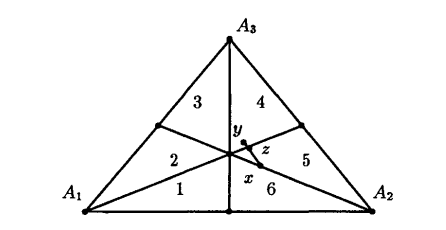
\includegraphics[width=\columnwidth,
 height=0.3\textheight]{./images/saari_triangle.png}
 \caption{Source: \textcite{nurmi2002voting}.}
 \label{fig:saari_nurmi}
\end{figure}

A further complication is a mismatch between the survey's
plurality result and the actual result of the first round. This is typical in
surveys, and might be due to strategic voting, social desirability bias (not
wanting to be seen as ``polarized''), or systematic refusal of part of the electorate
to answer the survey. Any imputation technique will reproduce this top choice discrepancy, thus I'll show directly the mismatch between the
imputation and the actual vote\footnote{In a further version of this working
  paper I'll show this directly, then contrast with the imputed data. They,
  thankfully, match,I'm just time-constrained.}. I ran the imputation algorithm
on the top 4 candidates, which means that in the sample the \(7.19\%\) that
voted for others is kept constant. The result after applying the algorithm is
Bolsonaro:Haddad:Ciro:Alckmin:Others = \(36.7.7\% : 17.3\% : 14.1\% :7.19\% \).
Thus, Bolsonaro and Haddad are undervoted in the sample, while Ciro and Alckmin
are overvoted\footnote{Remember the actual result was
  Bolsonaro:Haddad:Ciro:Alckmin:Others = \(46.3:29.28:12.47:4.76:7.19 \).}. If
we were simply transferring the top choices from over-voted to under-voted we
could simply, say, transfer Alckmin \(\rightarrow\) Bolsonaro and Ciro \(\rightarrow\) Hadddad.
However, there are 24 permutations of the top 4 candidates, with 6 for each
candidate in which they are the top alternative. This gives leeway to many
possible transfers. I have designed an algorithm, described in Appendix
\ref{appendix:transfer}, that, while respecting who can transfer and who needs
votes, respects the Kemeny's Distance between the rankings and picked the
transferred table that minimizes the euclidean distance between the inferred
table and the actual election. Two such inferred tables lead to the following
proportion: Bolsonaro:Haddad:Ciro:Alckmin:Others =
\(46.19:29.32:12.51:4.77:7.19 \). Since the application of electoral procedures
to those tables leads to qualitatively similar results, I'll just present the
results for one of them. The results for the other is in Appendix
\ref{appendix:transfer2_results}

\section{Results}
The inferred rankings\footnote{The whole table is shown in Appendix \ref{appendix:inferred1}.} are summarized in Figure \ref{fig:counts}. Indeed, the candidates that went to the second round were the most divisive ones. Ciro, however, could be considered more inclusive than Alckmin, since the proportion of last choices within Alckmin's subset of voters is higher than Ciro's. However, there is also a relevant distinction among the divisive candidates: Haddad's rejection was higher than his support, while the opposite held for Bolsonaro.

\begin{figure}[H]
 \centering
 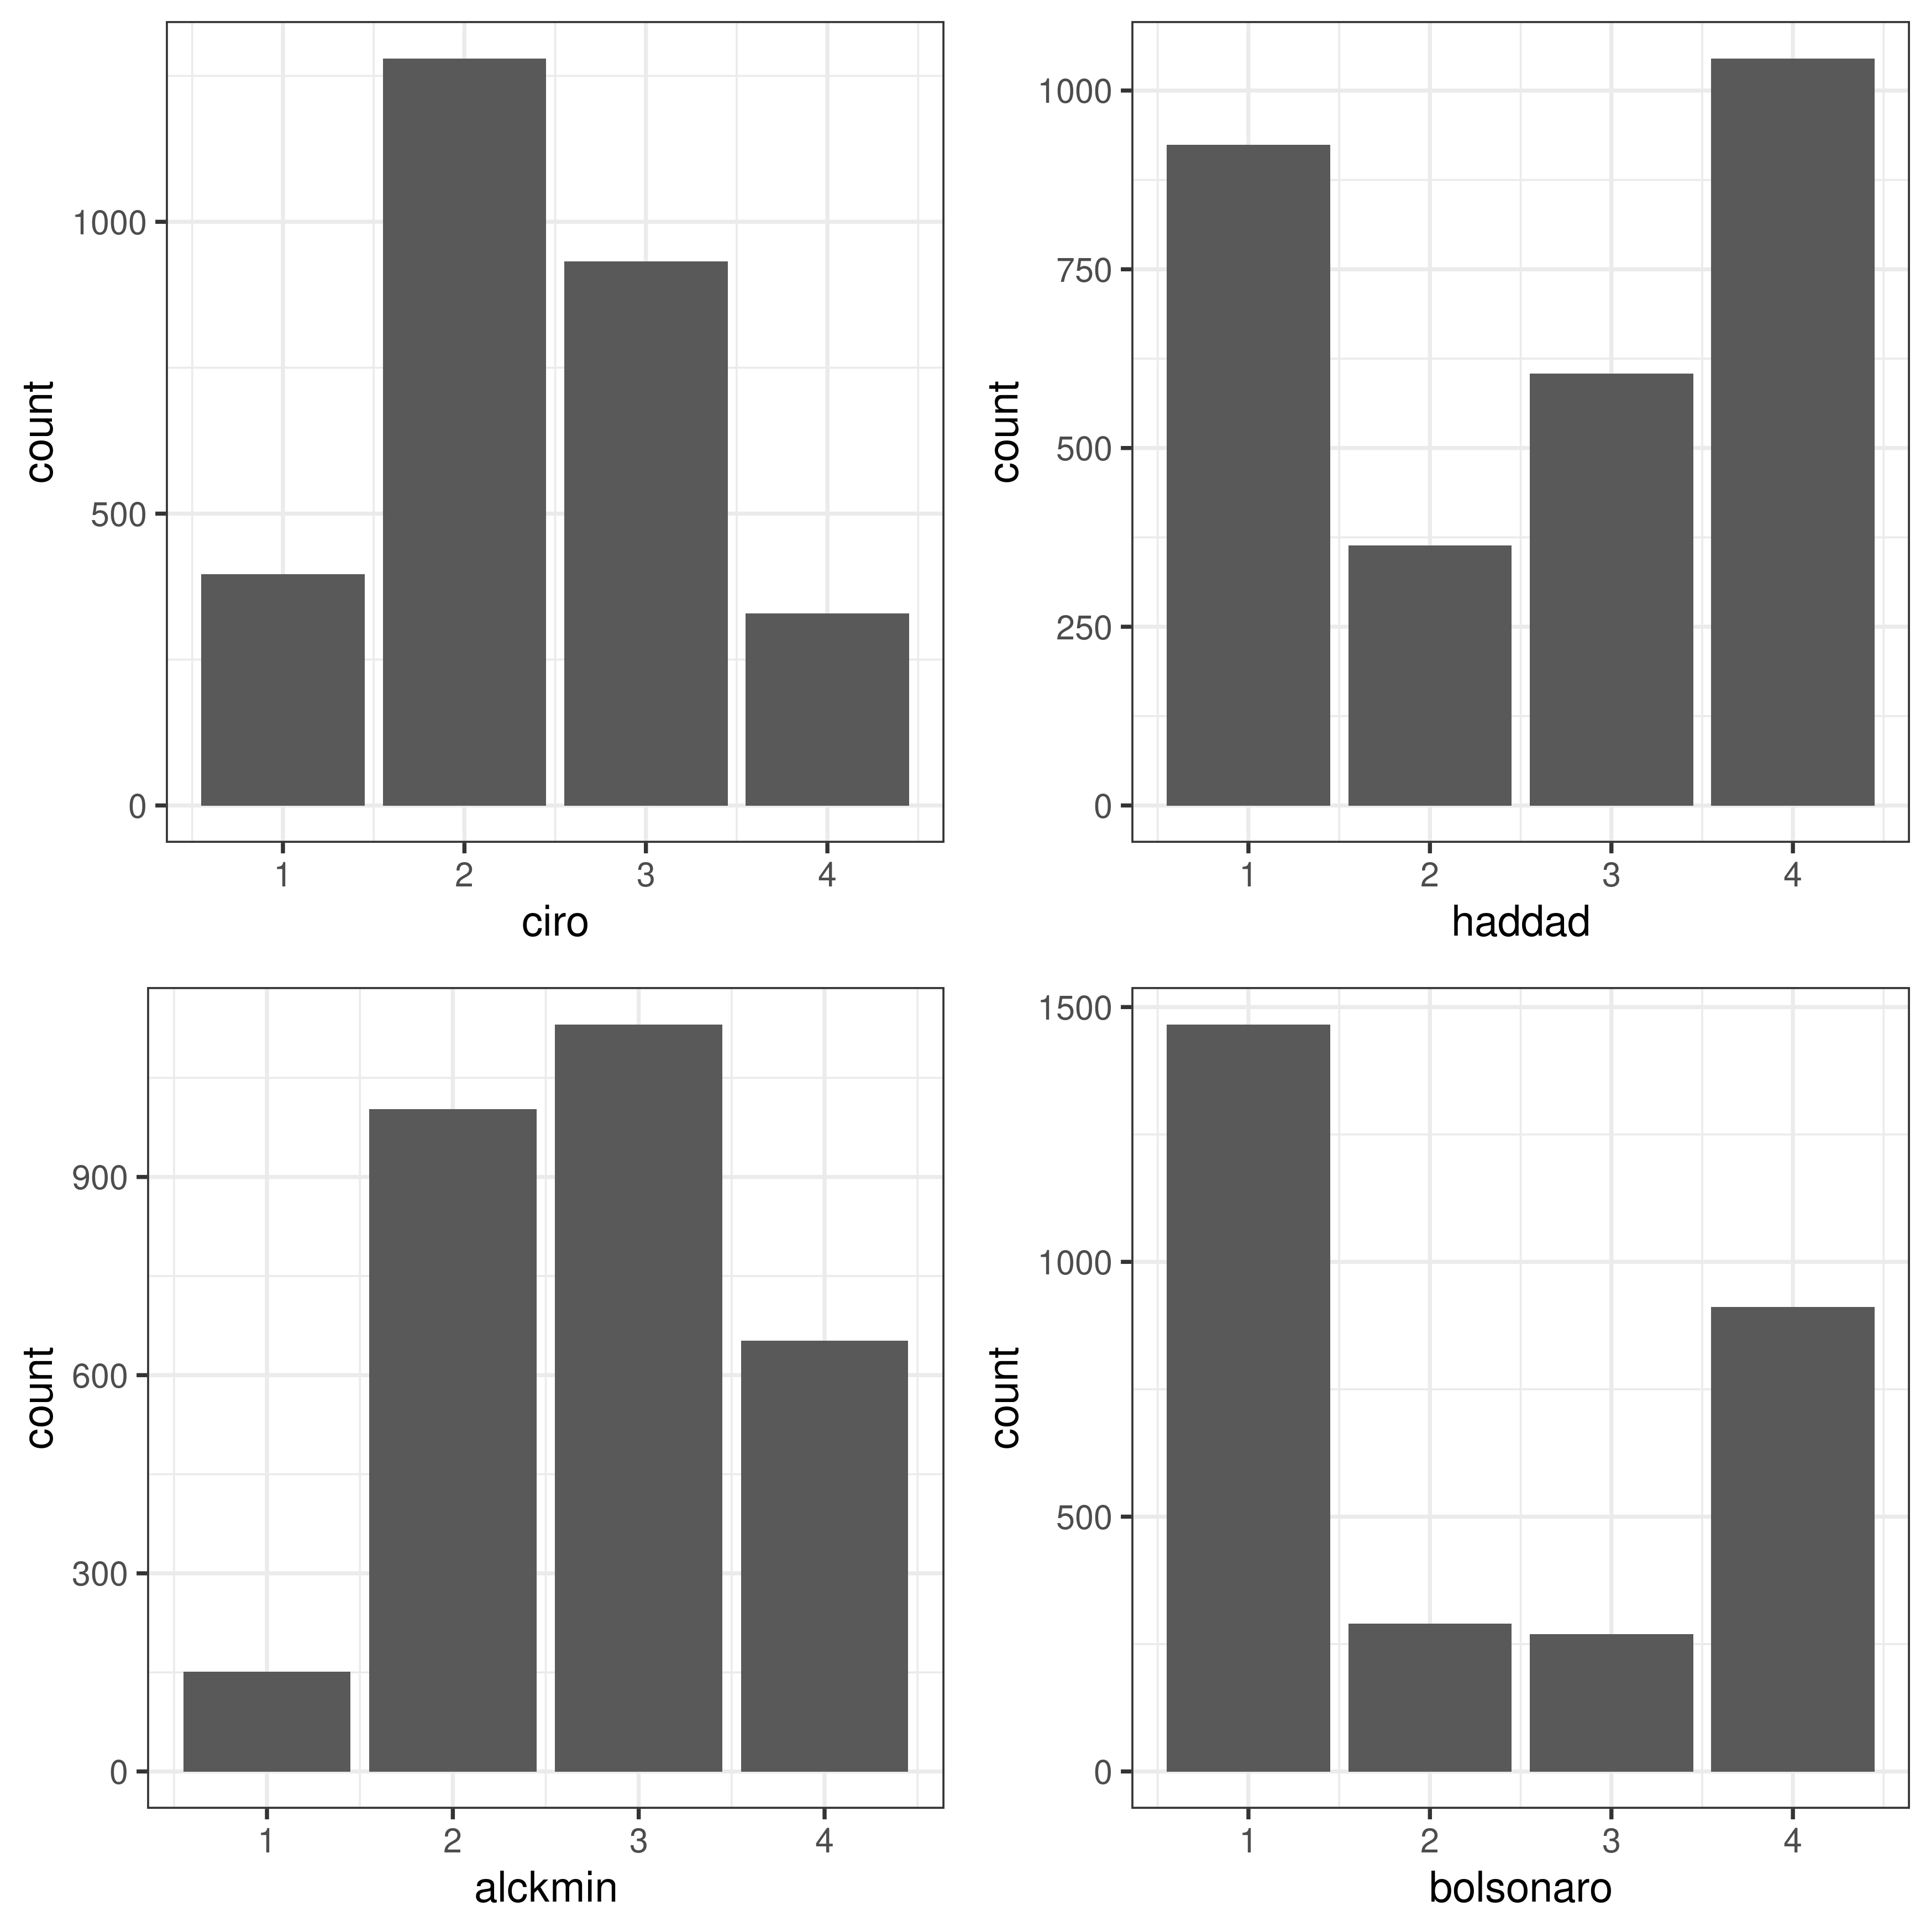
\includegraphics[width=0.8\columnwidth,
 height=0.5\textheight]{./images/corrected1_indexes_plot.png}
 \caption{Frequency candidates appear at each position}
 \label{fig:counts}
\end{figure}

But what does this support distribution mean from the point of view of the Borda and Condorcet procedures? Table \ref{tbl:tab1} shows what we can infer from the imputed data. Despite being a divisive candidate, Bolsonaro would have won in all pairwise majority comparisons against any of the other top candidates. Haddad, however, would have lost against Ciro, who would only have lost against Bolsonaro. Unlike what was widely believed at the time, and was the motto of  his campaign, Ciro most likely would not have won against Bolsonaro in a second round. He was not the ``anti-Bolsonaro'', but merely an ``anti-Haddad'', together with Bolsonaro. Alckmin, the candidate with the longest television time and the broadest supporting coalition would have lost against any other top candidates. He was the Condorcet Loser in the top set. The same pattern is reflected in the Borda Scores: Bolsonaro > Ciro > Haddad > Alckmin.


% latex table generated in R 4.2.1 by xtable 1.8-4 package
% Thu Dec  1 21:18:51 2022
\begin{table}[h]
\begin{subtable}[h]{0.4\textwidth}
\centering
\begin{tabular}{rrrrr}
  \hline
 & alckmin & bolsonaro & ciro & haddad \\
  \hline
alckmin & 0 & -1 & -1 & -1 \\
  bolsonaro & 1 & 0 & 1 & 1 \\
  ciro & 1 & -1 & 0 & 1 \\
  haddad & 1 & -1 & -1 & 0 \\
   \hline
\end{tabular}
\caption{Pairwise Majority Comparisons}
\label{tbl:subtab1}
\end{subtable}
\hfill
\begin{subtable}[h]{0.4\textwidth}
  \centering
\begin{tabular}{rr}
  \hline
 & borda score \\
  \hline
alckmin & 6527 \\
  bolsonaro & 8185 \\
  ciro & 7617 \\
  haddad & 7041 \\
   \hline
\end{tabular}
\caption{Borda scores}
\label{tbl:subtab2}
\end{subtable}
\caption{Borda and Condorcet results for final inferred ranking 1}
\label{tbl:tab1}
\end{table}


\begin{figure}[H]
 \centering
 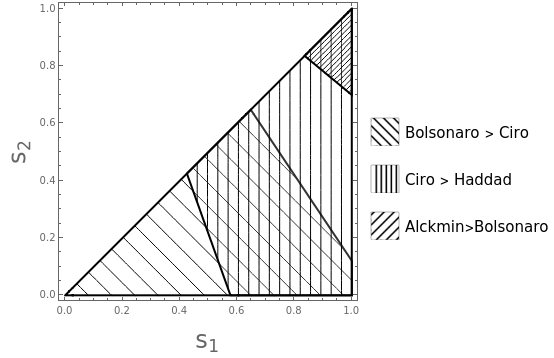
\includegraphics[width=\columnwidth,
 height=0.3\textheight]{./images/positional_results.png}
 \caption{Source: \textcite{nurmi2002voting}.}
 \label{fig:positional4c}
\end{figure}



\begin{table}
  \centering
  \begin{tabular}{rr}
    \hline\hline
    \textbf{candidates} & \textbf{\(w_s\) tallies} \\
    Alckmin & 0.3415*\(s\_1\) + 0.385*\(s\_2\) + 0.0514 \\
    Bolsonaro & 0.0988*\(s\_1\) + 0.0919*\(s\_2\) + 0.499 \\
    Ciro & 0.4358*\(s\_1\) + 0.3173*\(s\_2\) + 0.1348 \\
    Haddad & 0.1238*\(s\_1\) + 0.2057*\(s\_2\) + 0.3147 \\\hline\hline
  \end{tabular}
  \caption{\(w_{s}\) vector of each top 4 candidate}
\end{table}


\begin{table}[]
    \centering
\begin{tabular}{|r|r|r|r|}
\hline
\textbf{candidates} & \textbf{antiplurality} & \textbf{vote for two} & \textbf{plurality} \\ \hline
Alckmin             & 0.7779                 & 0.3929                & 0.0514             \\ \hline
Bolsonaro           & 0.6897                 & 0.5978                & 0.499              \\ \hline
Ciro                & 0.8879                 & 0.5706                & 0.1348             \\ \hline
Haddad              & 0.6442                 & 0.4385                & 0.3147             \\ \hline
\end{tabular}
\caption{Tallies for boundary positional methods (dropping ``Others'' )}
\end{table}




\begin{table}[]
  \centering
\begin{tabular}{|r|r|r|r|r|}
\hline
\textbf{candidates} & \textbf{alckmin} & \textbf{bolsonaro} & \textbf{ciro} & \textbf{haddad} \\ \hline
alckmin             & -             & 0.05               & 0.0           & 0.25            \\ \hline
bolsonaro           & 0.95             & -            & 0.69          & 1.0             \\ \hline
ciro                & 1.0              & 0.31               & -           & 0.76            \\ \hline
haddad              & 0.75             & 0.0                & 0.24          & -            \\ \hline
\end{tabular}
\caption{Percentage of positional victories of row against column}
\end{table}








However, neither the CW nor the family of positional voting methods are, in
general, Independent of the Alternative Set\parencite{kaminski2015empirical}.
That is if we drop or add candidates, the ``social'' ranking might change
without respecting the ordering of the baseline set of alternatives. Consider
the Borda-induced social ranking in this case: Bolsonaro > Ciro > Haddad >
Alckmin. If by dropping Alckmin, the ranking changes to Ciro > Bolsonaro >
Haddad, then the Borda Count, in this case, would be inducing a ``paradoxical.''
result. In Figure \ref{fig:c1dropping} we consider alternative scenarios by
dropping one of the top 4 candidates. Not only can we determine if there is any ``alternative set stability'', but also take into account the positional stability of the result.

In terms of alternative set stability, the positional voting
procedures are eminently well-behaved in this case. The only reversal seems to be the
antiplurality ranking if Haddad had dropped. In this case, Figure
\ref{fig:c1dropping} (d), the antiplurality ranking was\footnote{\texts have to
  confirm that. I even have the code for it written somewhere.} Ciro > Alckmin >
Bolsonaro > Haddad, but now the ranking is Ciro > Bolsonaro > Alckmin. The
reason is that Haddad's votes were most likely transferred more to Ciro
than to Alckmin. The antiplurality point, however, is very close to a tie
between Bolsonaro and Alckmin, which means this can also be an artifact
of sampling uncertainty.


What about positional stability? Notice that in all scenarios where Bolsonaro is still in the alternative set he would have been both the plurality and the Borda winner, and most positional voting methods would have elected him. The only counterfactual positional results in which he would not have been elected is if a voting procedure that emphasized rejection had been used, and Ciro would then have been elected. Those scenarios, however, are in these cases, Figure \ref{fig:c1dropping} (a,c,d), always a minority. His victory, thus, was not a fluke, or an artifact of institutional technology. Not only he would have won under both Borda and Condorcet methods, but his victory was also stable under both alternative sets of alternatives and alternative positional methods. This amounts to a hoop test falsification of the idea that divisive closet authoritarians are an artifact of the current decision procedures \parencite{mahoney2006tale}. It may well be true in the USA, but does not hold in general. Even though electoral systems based on just the first positions of citizens' preferences do ignore, by definition, the distribution of support the candidates have throughout the whole rankings, and we could expect that divisive candidates would fare worse under informationally richer decision procedures, a divisive candidate can still be a CW with high positional stability. Therefore, highly polarized scenarios can lead to the election of a divisive candidate regardless of which decision procedure is being used.



However, figure \ref{fig:c1dropping} (c) presents an interesting scenario.
Though, as expected, Haddad would have been the plurality winner\footnote{As
  shown in Figure \ref{fig:c2dropping} in Appendix
  \ref{appendix:transfer2_results}, this is a case in which the vote transfers
  differ. In the alternative vote transfer, in this scenario, Ciro would have
  tied with Haddad in the plurality case, but would have won under all other
  positional voting methods.}, now his victory would not have been positionally
stable. In Table \ref{tbl:subtab1} it was shown that Ciro would have
beaten him with a majority pairwise comparison, which gives credence to affirming
that Ciro would have won under a majority with run-off system. In this scenario
the most inclusive candidate would have been elected. Within Latin America,
Brazil sticks out for its lack of transitional justice
\parencite{nalepa2022after}. The remnants of the old regime were never punished,
and Bolsonaro is an instance of such group. It is no coincidence after being
elected he assigned \(70\%\) more military to public administration positions
traditionally held by civilians. Or that in his term the army re-emerged in the
country as a prominent political actor, with generals feeling comfortable to
periodically remind the civil society that the military forces function as a
``moderating power''\footnote{As the Emperor used to do before the
  Independence.} in the political system. If wolves in sheep clothes are at the
door, as characterized by \textcite{chiopris2021wolf}, then maybe citizens
should not leave it open for them. This leads to an empirical implication for
the subset of transitional democracies (those that are still in the process of
democratization \parencite{svolik2008authoritarian}): the election of closet
authoritarians is more probable in countries that have a military dictatorship
past, but didn't go through a transitional justice process
\parencite{geddes1999we}. Testing it is a subject of future studies.




% Case a:
% - plurality bhc
% - antiplurality cbh
% - borda: bch

% Case b:
% - plurality: hca
% - borda: cha
% - antiplurality: c(ha)

% Case c:
% - plurality: bha
% - antiplurality: abh
% - borda: bha

% Case d:
% - plurality: bca
% - antiplurality: cba
% - borda: bca

   \begin{figure}[H]
        \centering
        \begin{subfigure}[b]{0.475\textwidth}
            \centering
            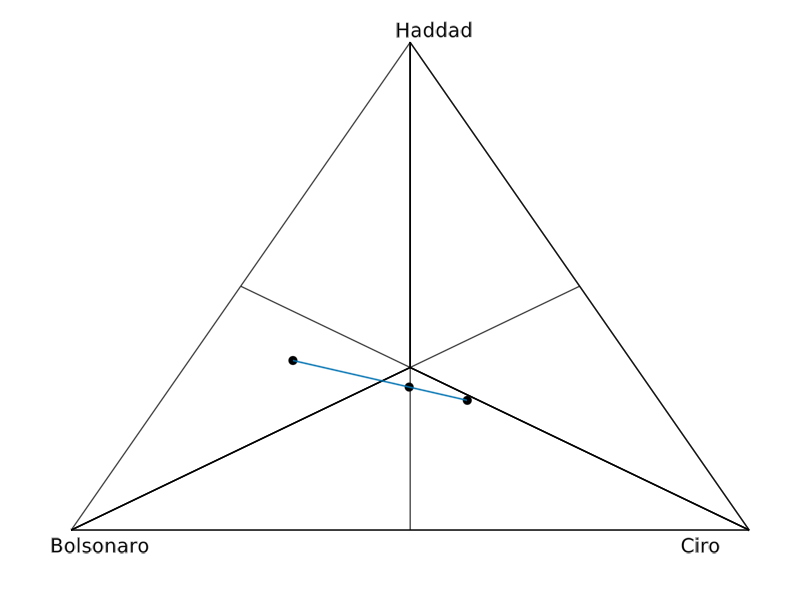
\includegraphics[width=\textwidth]{./images/cw1_nota.png}
             \caption{}%
            % {{\small Network 1}}
            \label{fig:notac1}
        \end{subfigure}
        \hfill
        \begin{subfigure}[b]{0.475\textwidth}
            \centering
            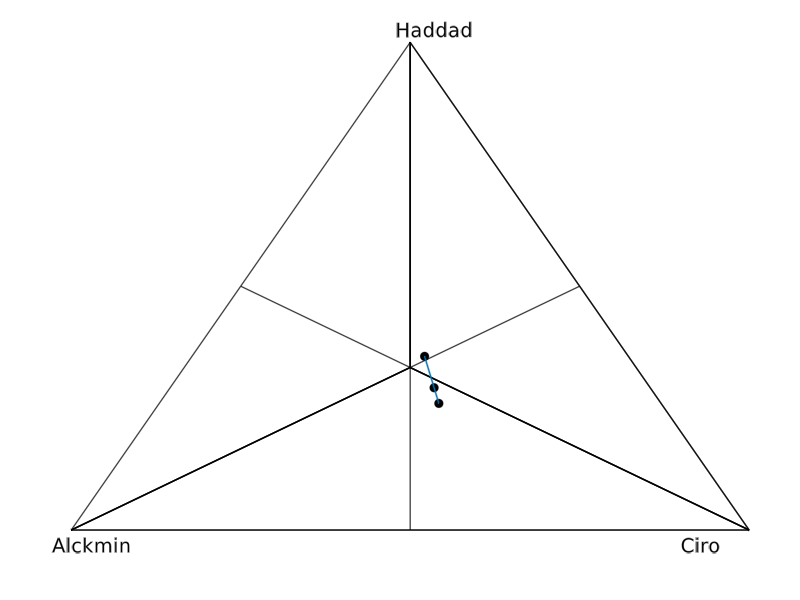
\includegraphics[width=\textwidth]{./images/cw1_notb.png}
             \caption{}%
            % {{\small Network 2}}
            \label{fig:notbc1}
        \end{subfigure}
        \vskip\baselineskip
        \begin{subfigure}[b]{0.475\textwidth}
            \centering
            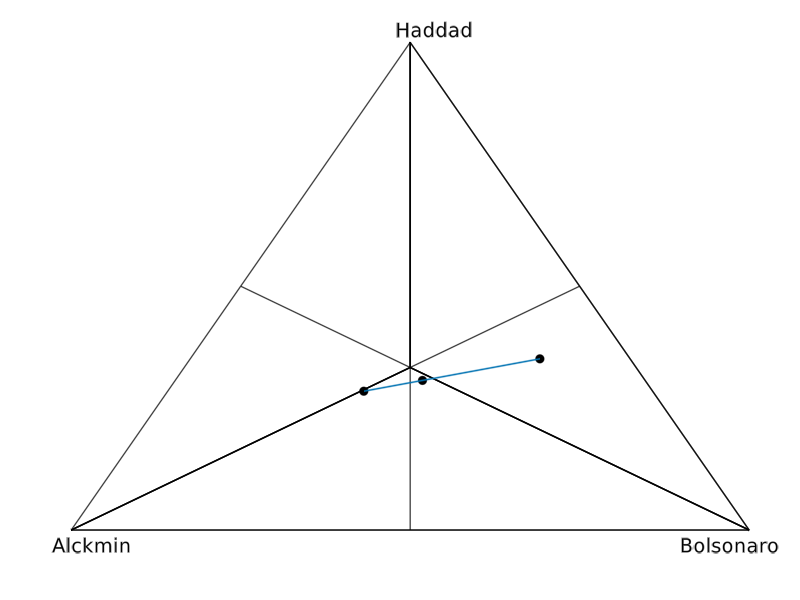
\includegraphics[width=\textwidth]{./images/cw1_notc.png}
            \caption{}%
            \label{fig:notbc1}
        \end{subfigure}
        \hfill
        \begin{subfigure}[b]{0.475\textwidth}
            \centering
            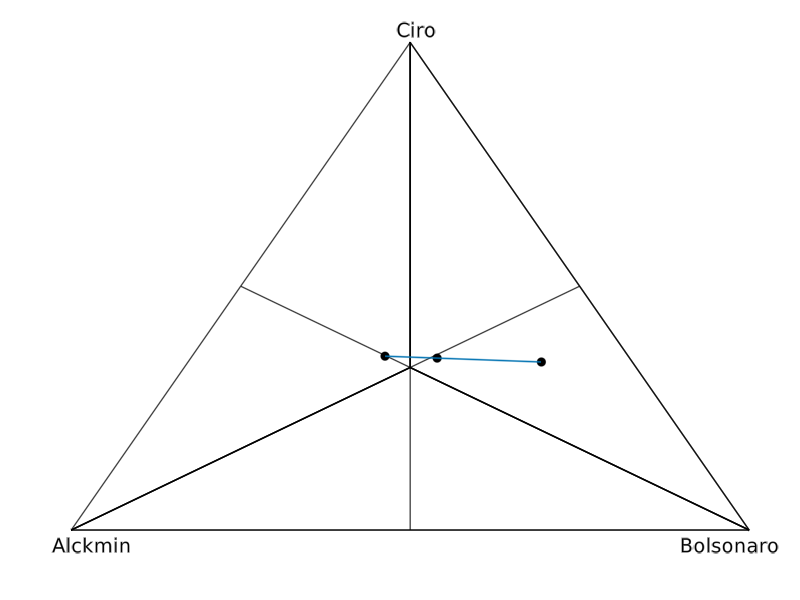
\includegraphics[width=\textwidth]{./images/cw1_noth.png}
             \caption{}%
            % {{\small Network 4}}
            \label{fig:notah1}
        \end{subfigure}
        \caption[  Positional results when dropping one candidate ]
        {\small Positional results after dropping one candidate }
        \label{fig:c1dropping}
    \end{figure}

    \textcolor{red}{I still intend to }:
    \begin{itemize}
      \item Elaborate on the statistical model, and show diagnostics for it;
      \item Implement the opened tetrahedron with its procedure hull. It will be the first empirical paper to do that;
      \item Implement a decomposition of the votes for 4 candidates. Again, it would be the first empirical paper to do that (Nurmi did that for 3 candidates);
      \item Do highschool geometry on the procedure line and give a measure to assertions such as : ``most positional methods would elect Bolsonaro in such scenario''
    \end{itemize}
\section{Conclusion}

The paper contributes to the analysis of the institutional robustness of
polyarchical systems, by considering credible alternative voting procedures'
outcomes and properties at a critical juncture in Brazil's political history. We
have demonstrated empirically that, contrary to established
theoretical expectations, Bolsonaro's victory was not caused by the decision
procedure.

The most glaring limitation of the paper is that agents adapt to new
institutional environments. By assuming a direct
translation between preferences and behavior we are ignoring strategic voting.
The percentage of strategic voting in a large scale election, however, is an
open empirical problem \parencite{straeten10_strat_sincer_heuris_votin_under,kawai2013inferring}. Nevertheless, a
combination of game-theoretic models with a simulation parameterized by the
inferred ranking distribution is a route of research that I intend to pursue.

The research used only one variable from the dataset, the pairwise
comparisons, to simulate alternative scenarios. However, socio-demographic
variables from the dataset could have been used to strengthen the data
imputation procedure. Speaking of imputation, simpler imputations, such as the
Impartial Culture assumption \parencite{regenwetter2006behavioral}, could have been
used as benchmarks to compare with the imputation through the bayesian mallows
model. Moreover, it is necessary to properly analyze the pattern of missingness
of pairwise comparisons. Roughly less than half of the dataset is constituted of
incomplete pairwise comparisons, and there might be valuable information on the
agent's preferences contained in patterns of missingness
\parencite{mcelreath2020statistical}.

Other voting procedures could have been used. Particularly, truncated positional
voting methods could have been directly applied to the raw data
\parencite{terzopoulou2021borda}. Moreover, we have been disregarding
indifference in the agent's preferences. Again, this is valuable information,
and it is known that forcing strict preferences when indifference exists leads
to artificial inflation of the profile inconsistency
\parencite{gehrlein2010impact}. Finally, though we have analyzed the four top
candidates, there is no direct relationship between the result of an election
with positional procedures when we have a subset of the alternatives vs when we
have the whole set of candidates \parencite{saari2001chaotic}. It is well known,
for instance, that the Borda Count violates WARP precisely because it is not
contraction-expansion consistent \parencite{schwartz2018cycles}. Nonetheless, we
expect that the results will not reverse, given that the bottom candidates could
be deemed irrelevant to most of the population (and as such, be tied in the
bottom of the rankings), and the patterns seen when dropping only one candidate.
This is a subject for a more thorough analysis, in any case. Finally, even
though we have analyzed scenarios in which candidates were removed, and
alternative voting procedures could have been used, it would be more realistic
to simulate the formation of coalitions and how voters would have reacted to
those. The assumption of a pure additive transfer of votes, implicit when we
removed candidates, is not necessarily true with coalitions, insofar voters of a
center-left candidate, for instance, could actually, vote for the center-right
candidate if they are alienated by an alliance with the Left, which in the case
of the election under scrutiny, was highly rejected, as shown in our analysis.


\printbibliography
\pagebreak
\appendix
\section{The vote transfer algorithm}\label{appendix:transfer}

 If we are to transfer from Alckmin to Bolsonaro we are lead to the problem of first
picking which ranking at the source should be chosen then which ranking at the
target should receive votes, while respecting how much the source has in excess
and how much the target needs\footnote{In a further version of this paper
  I'll describe this with the help of a pseudo-code of the algorithm.}. A
natural sorting of which ranking should be the source is the position of
Bolsonaro in the ranking. We start with rankings in which he is in the second
position ((Alckmin, Bolsonaro, Ciro, Haddad), (Alckmin, Bolsonaro, Haddad,
Ciro)), then third position ((Alckmin, Ciro, Bolsonaro, Haddad), (Alckmin,
Haddad, Bolsonaro, Ciro )), then last position ((Alckmin, Ciro, Haddad,
Bolsonaro), ((Alckmin, Haddad, Ciro, Bolsonaro))). Let's call those sets the
sorted rankings sets. Suppose we picked a source ranking from the first sorted
rankings set. What should be the target ranking, among the rankings which have
Bolsonaro as the first choice? We transfer to the ranking that has minimal
Kemeny's distance to the source ranking \parencite{nurmi2002voting}. The Kemeny
distance counts the number of transpositions (switching of pairs) needed to go
from one permutation to another permutation. Thus, we transfer from the source
ranking the min(number of votes the source ranking has, the total number of
votes the under-voted needs, the total number of votes the over-voted can give).
We update the source ranking frequency, the target ranking frequency, the total
number of votes the under-voted needs, and the total number of votes the
over-voted can give. If the under-voted doesn't need any other votes we stop and
go to another over-voted \(\to\) under-voted transfer. If not we check if the
over-voted can still transfer votes to the current target under-voted. If yes we
pick another source ranking in the sorted rankings sets and repeat until either
the source has run out of votes it can given or the target has received enough
votes. If not we go to another over-voted \(\to\) under-voted transfer. In the end, this leads to 24 possible transfer sequences from over-voted
to under-voted. One possible sequence is Alckmin \(\to\) Bolsonaro, then Alckmin
\(\to\) Haddad, then Ciro \(\to\) Haddad, then Ciro \(\to\) Bolsonaro. Another
possible sequence is  Alckmin \(\to\) Bolsonaro, then Alckmin \(\to\) Haddad, then
Ciro \(\to\) Bolsonaro, then Ciro \(\to\) Haddad. This leads to 6 transfers that
minimize the euclidean distance between the inferred plurality result and actual
result of the first round. However, there are actually two equivalence classes
among those 6: 3 have the same proportion for each ranking, while the other 3
have the same proportion for each ranking. The new inferred proportion for both
classes is: Bolsonaro:Haddad:Ciro:Alckmin:Others =
\(46.19:29.32:12.51:4.77:7.19 \).

\section{Inferred Ranking Table} \label{appendix:inferred1}


\begin{table}[H]
  \centering
\begin{tabular}{|r|r|}
\hline
\textbf{ranking vectors}                           & \textbf{percentage} \\ \hline
haddad \textgreater ciro \textgreater alckmin \textgreater bolsonaro & 17.19                                \\ \hline
bolsonaro \textgreater alckmin \textgreater ciro \textgreater haddad & 13.99                                \\ \hline
bolsonaro \textgreater ciro \textgreater alckmin \textgreater haddad & 13.72                                \\ \hline
bolsonaro \textgreater ciro \textgreater haddad \textgreater alckmin & 8.85                                 \\ \hline
haddad \textgreater alckmin \textgreater ciro \textgreater bolsonaro & 7.12                                 \\ \hline
bolsonaro \textgreater haddad \textgreater ciro \textgreater alckmin & 6.26                                 \\ \hline
ciro \textgreater alckmin \textgreater haddad \textgreater bolsonaro & 5.04                                 \\ \hline
bolsonaro \textgreater alckmin \textgreater haddad \textgreater ciro & 4.36                                 \\ \hline
haddad \textgreater ciro \textgreater bolsonaro \textgreater alckmin & 3.51                                 \\ \hline
alckmin \textgreater bolsonaro \textgreater ciro \textgreater haddad & 2.79                                 \\ \hline
bolsonaro \textgreater haddad \textgreater alckmin \textgreater ciro & 2.72                                 \\ \hline
ciro \textgreater alckmin \textgreater bolsonaro \textgreater haddad & 2.72                                 \\ \hline
ciro \textgreater bolsonaro \textgreater alckmin \textgreater haddad & 2.04                                 \\ \hline
ciro \textgreater haddad \textgreater alckmin \textgreater bolsonaro & 1.67                                 \\ \hline
haddad \textgreater bolsonaro \textgreater ciro \textgreater alckmin & 1.57                                 \\ \hline
alckmin \textgreater bolsonaro \textgreater haddad \textgreater ciro & 1.5                                  \\ \hline
ciro \textgreater haddad \textgreater bolsonaro \textgreater alckmin & 1.19                                 \\ \hline
haddad \textgreater bolsonaro \textgreater alckmin \textgreater ciro & 1.16                                 \\ \hline
haddad \textgreater alckmin \textgreater bolsonaro \textgreater ciro & 0.92                                 \\ \hline
ciro \textgreater bolsonaro \textgreater haddad \textgreater alckmin & 0.82                                 \\ \hline
alckmin \textgreater haddad \textgreater bolsonaro \textgreater ciro & 0.54                                 \\ \hline
alckmin \textgreater ciro \textgreater bolsonaro \textgreater haddad & 0.31                                 \\ \hline
\end{tabular}
\caption{Inferred rankings}
\label{lab:inferred1}
\end{table}


\section{The results for the other inferred table}\label{appendix:transfer2_results}

\begin{table}[H]
  \centering
\begin{tabular}{|r|r|}
\hline
\textbf{ranking vectors}                           & \textbf{percentage} \\ \hline
bolsonaro \textgreater alckmin \textgreater ciro \textgreater haddad & 13.99                                \\ \hline
bolsonaro \textgreater ciro \textgreater haddad \textgreater alckmin & 13.69                                \\ \hline
haddad \textgreater ciro \textgreater alckmin \textgreater bolsonaro & 12.36                                \\ \hline
bolsonaro \textgreater ciro \textgreater alckmin \textgreater haddad & 11.1                                 \\ \hline
haddad \textgreater alckmin \textgreater ciro \textgreater bolsonaro & 9.33                                 \\ \hline
haddad \textgreater ciro \textgreater bolsonaro \textgreater alckmin & 6.13                                 \\ \hline
ciro \textgreater alckmin \textgreater haddad \textgreater bolsonaro & 5.04                                 \\ \hline
bolsonaro \textgreater alckmin \textgreater haddad \textgreater ciro & 4.36                                 \\ \hline
bolsonaro \textgreater haddad \textgreater ciro \textgreater alckmin & 4.05                                 \\ \hline
alckmin \textgreater bolsonaro \textgreater ciro \textgreater haddad & 2.79                                 \\ \hline
bolsonaro \textgreater haddad \textgreater alckmin \textgreater ciro & 2.72                                 \\ \hline
ciro \textgreater alckmin \textgreater bolsonaro \textgreater haddad & 2.72                                 \\ \hline
ciro \textgreater bolsonaro \textgreater alckmin \textgreater haddad & 2.04                                 \\ \hline
ciro \textgreater haddad \textgreater alckmin \textgreater bolsonaro & 1.67                                 \\ \hline
haddad \textgreater bolsonaro \textgreater ciro \textgreater alckmin & 1.57                                 \\ \hline
alckmin \textgreater bolsonaro \textgreater haddad \textgreater ciro & 1.5                                  \\ \hline
ciro \textgreater haddad \textgreater bolsonaro \textgreater alckmin & 1.19                                 \\ \hline
haddad \textgreater bolsonaro \textgreater alckmin \textgreater ciro & 1.16                                 \\ \hline
haddad \textgreater alckmin \textgreater bolsonaro \textgreater ciro & 0.92                                 \\ \hline
ciro \textgreater bolsonaro \textgreater haddad \textgreater alckmin & 0.82                                 \\ \hline
alckmin \textgreater haddad \textgreater bolsonaro \textgreater ciro & 0.54                                 \\ \hline
alckmin \textgreater ciro \textgreater bolsonaro \textgreater haddad & 0.31                                 \\ \hline
\end{tabular}
\caption{Second minimizing inferred rankings - one ranking got 0 votes after the transfer}
\end{table}



\begin{figure}[H]
 \centering
 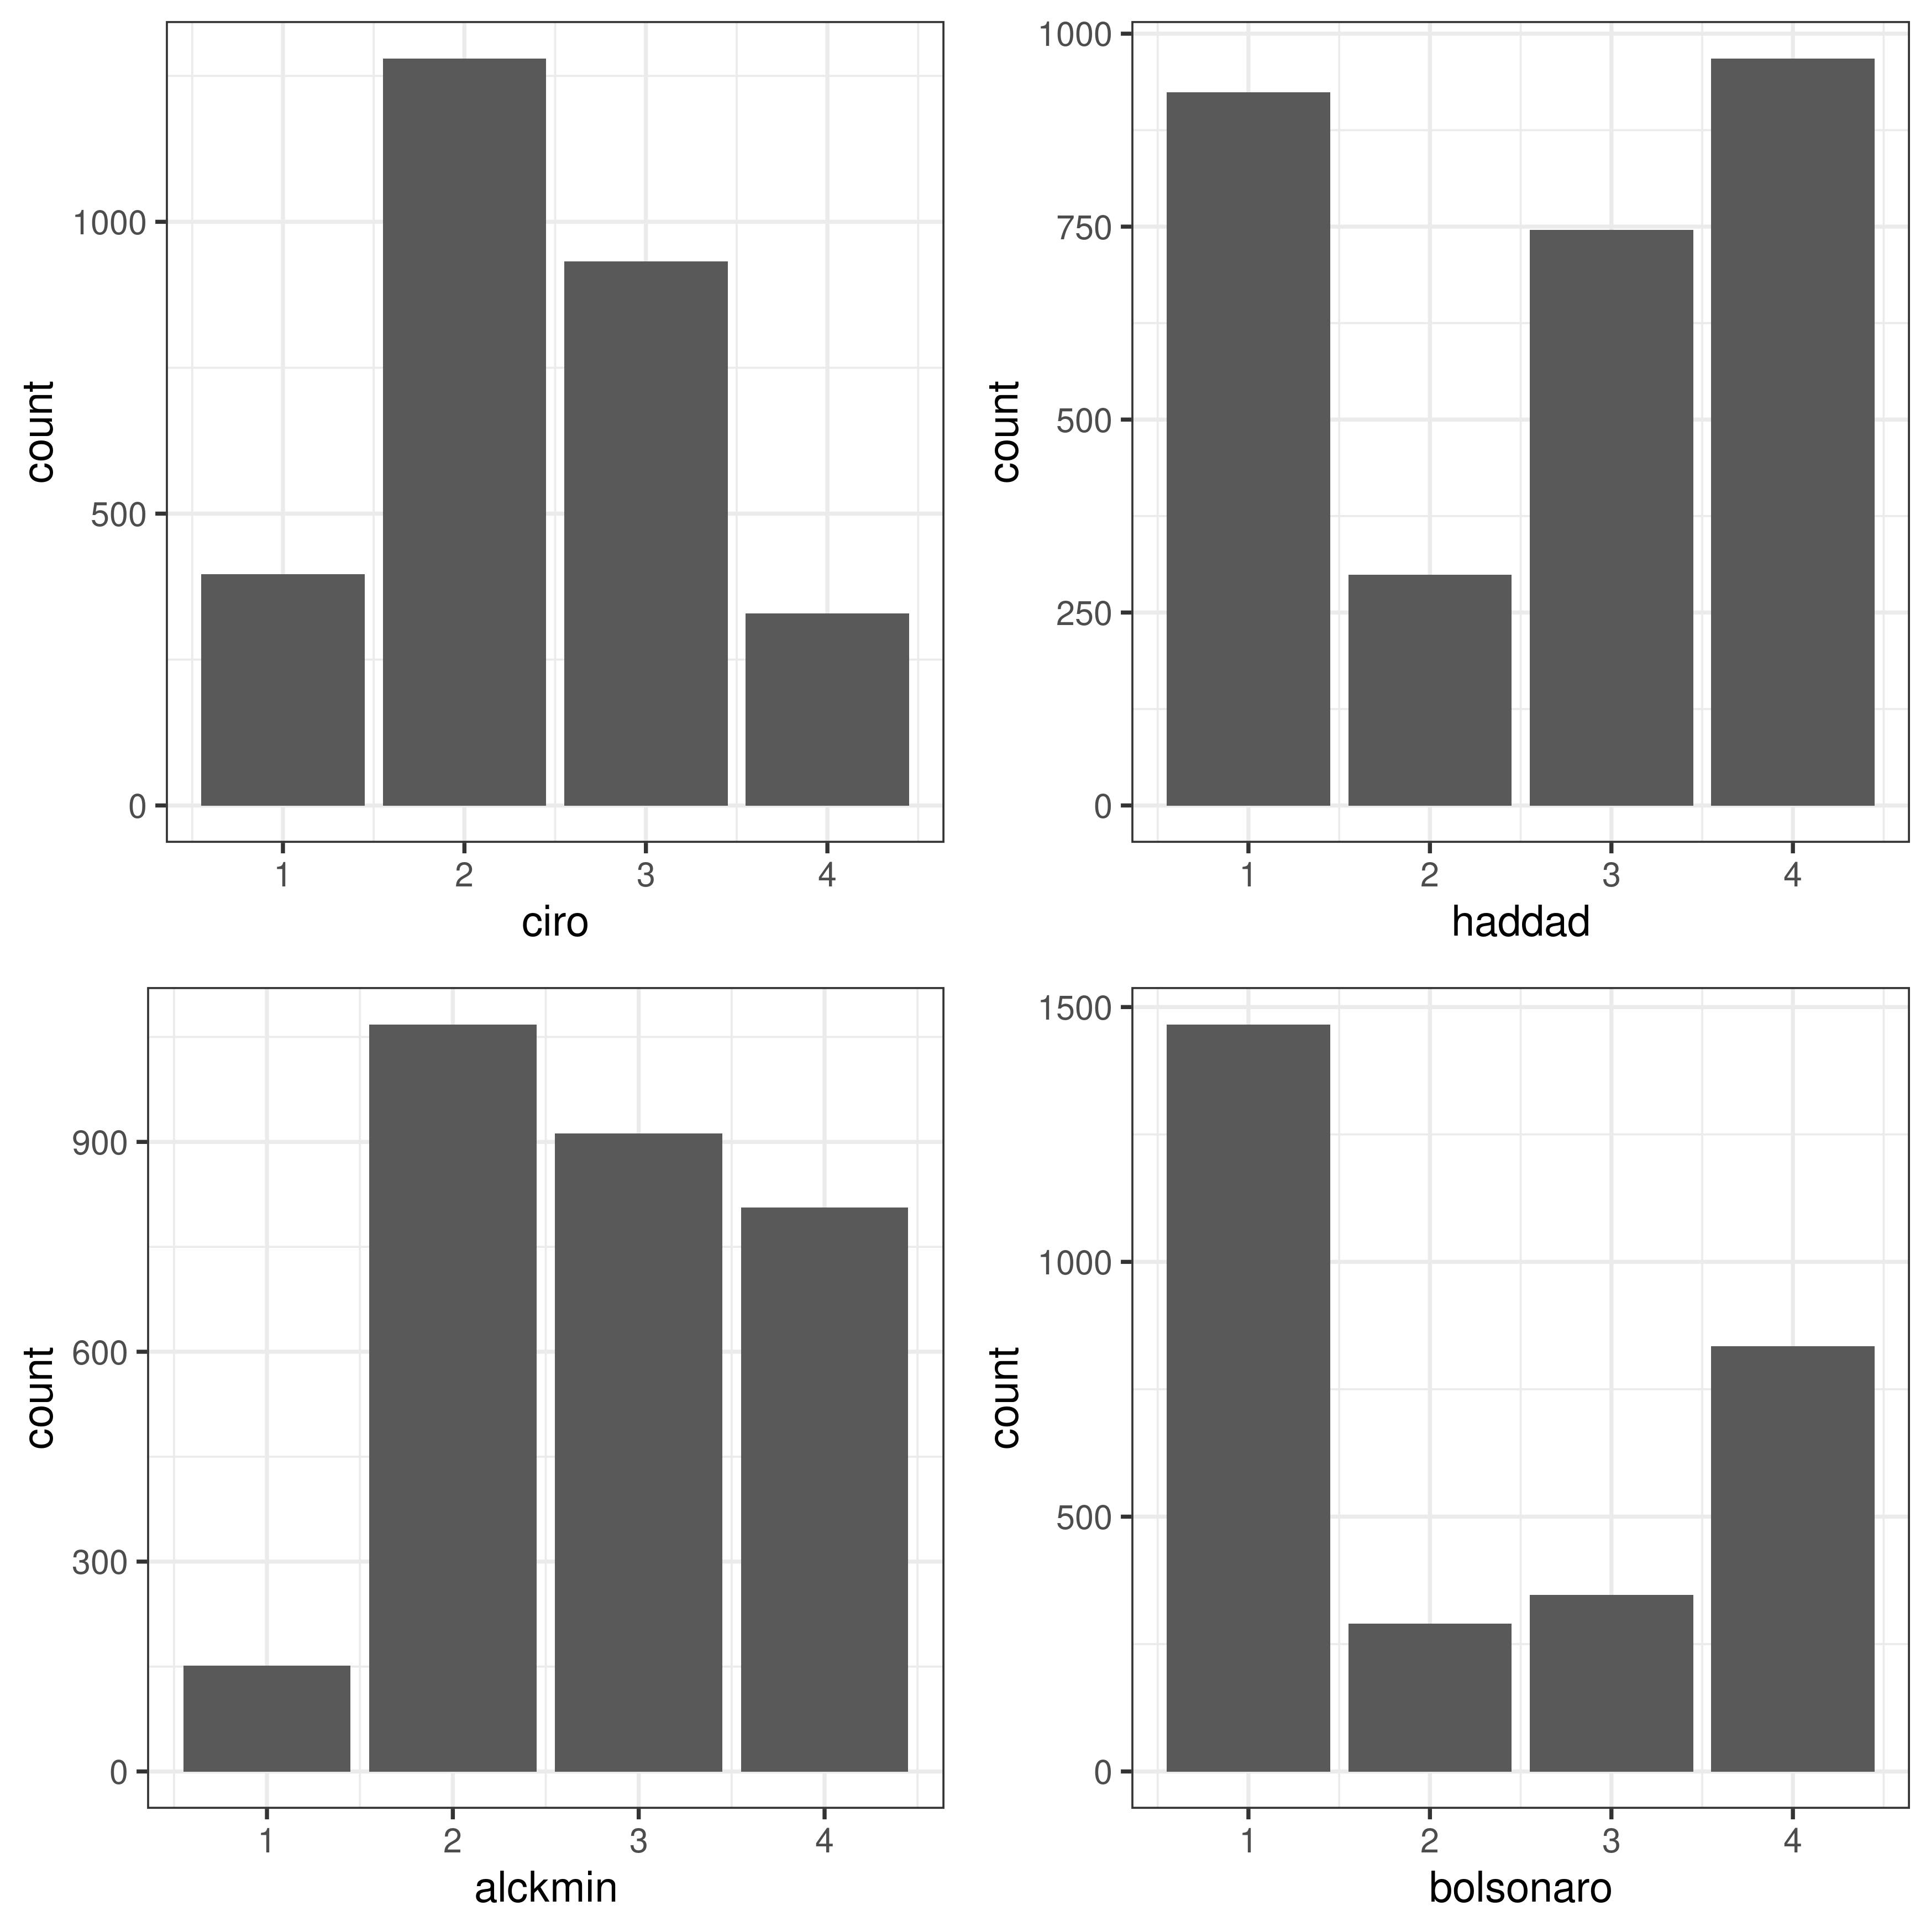
\includegraphics[width=0.8\columnwidth,
 height=0.5\textheight]{./images/corrected2_indexes_plot.png}
 \caption{Number of times candidates appear at each position - final ranking 2}
\end{figure}

% latex table generated in R 4.2.1 by xtable 1.8-4 package
% Thu Dec  1 21:18:52 2022
\begin{table}[H]
  \begin{subtable}[h]{0.4\textwidth}
    \centering
\begin{tabular}{rrrrr}
  \hline
 & alckmin & bolsonaro & ciro & haddad \\
  \hline
alckmin & 0 & -1 & -1 & -1 \\
  bolsonaro & 1 & 0 & 1 & 1 \\
  ciro & 1 & -1 & 0 & 1 \\
  haddad & 1 & -1 & -1 & 0 \\
   \hline
\end{tabular}
\caption{Pairwise Majority Comparisons }
\end{subtable}
\hfill
\begin{subtable}[h]{0.4\textwidth}
\centering
\begin{tabular}{rr}
  \hline
 & borda2\$other\_info\$count\_max \\
  \hline
alckmin & 6438 \\
  bolsonaro & 8262 \\
  ciro & 7617 \\
  haddad & 7053 \\
   \hline
\end{tabular}
\caption{Borda scores}
\end{subtable}
\caption{Borda and Condorcet results for final inferred ranking 2}
\end{table}


   \begin{figure*}
        \centering
        \begin{subfigure}[b]{0.475\textwidth}
            \centering
            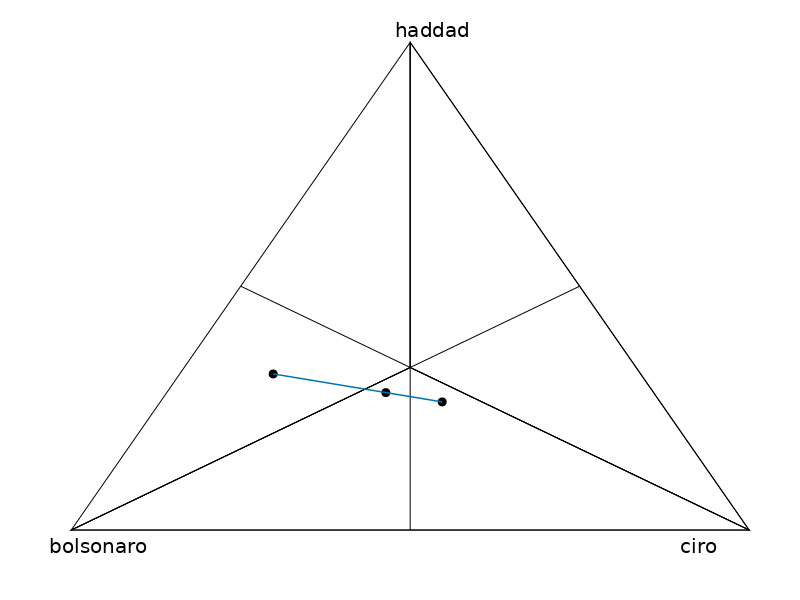
\includegraphics[width=\textwidth]{./images/cw2_nota.png}
             \caption{}%
            % {{\small Network 1}}
            \label{fig:notac2}
        \end{subfigure}
        \hfill
        \begin{subfigure}[b]{0.475\textwidth}
            \centering
            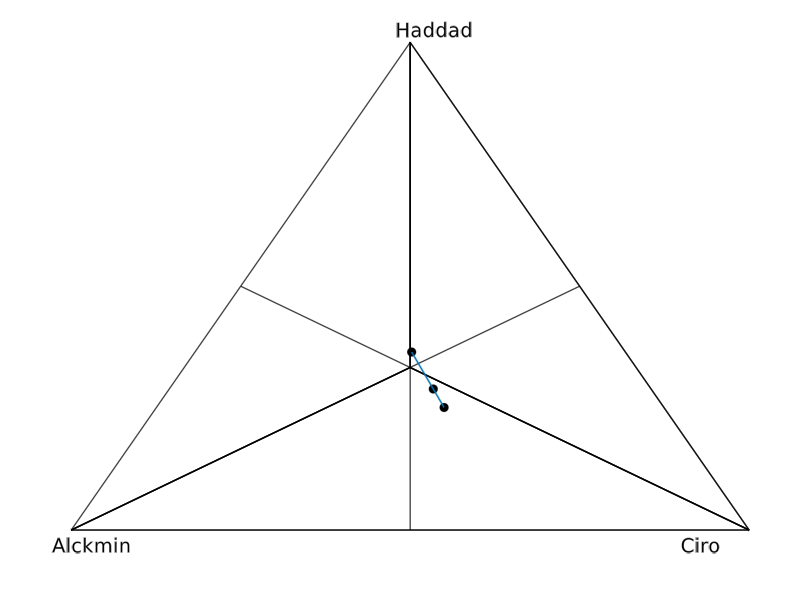
\includegraphics[width=\textwidth]{./images/cw2_notb.png}
             \caption{}%
            % {{\small Network 2}}
            \label{fig:notbc2}
        \end{subfigure}
        \vskip\baselineskip
        \begin{subfigure}[b]{0.475\textwidth}
            \centering
            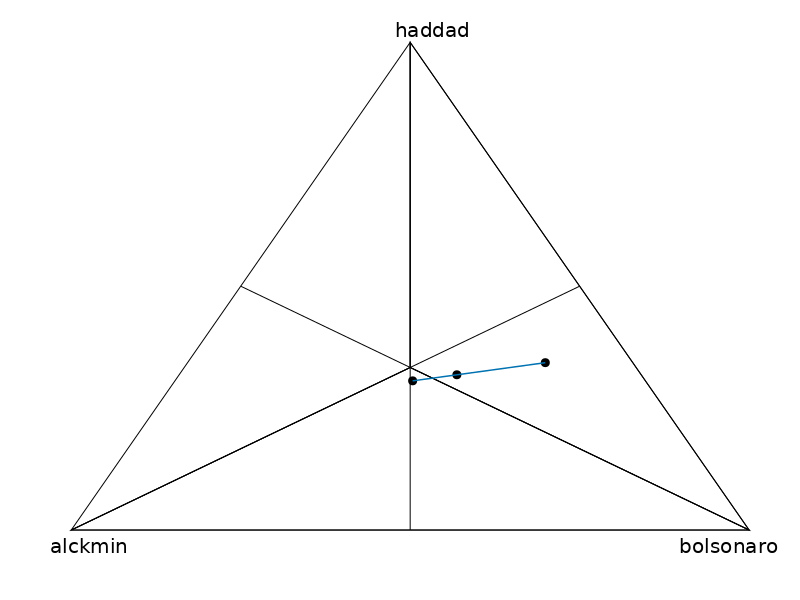
\includegraphics[width=\textwidth]{./images/cw2_notc.png}
            \caption{}%
%            {{\small Network 3}}
            \label{fig:notbc2}
        \end{subfigure}
        \hfill
        \begin{subfigure}[b]{0.475\textwidth}
            \centering
            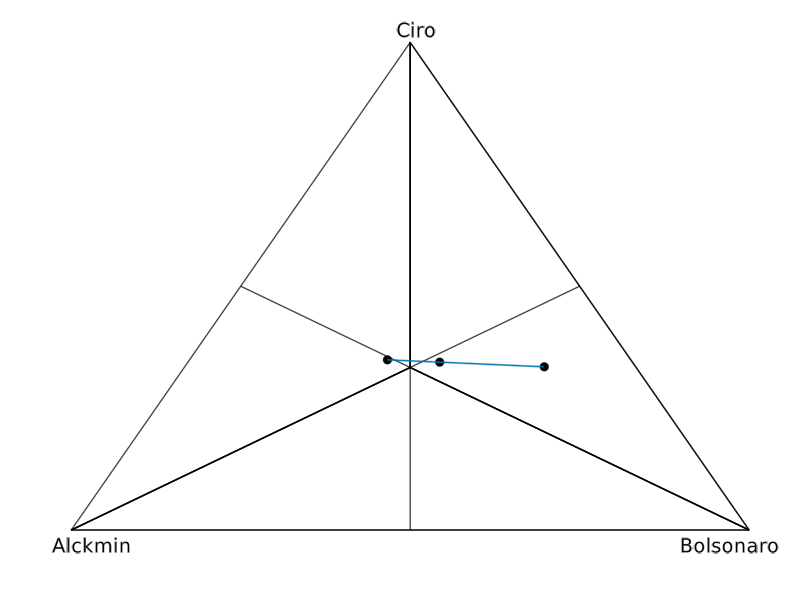
\includegraphics[width=\textwidth]{./images/cw2_noth.png}
             \caption{}%
            % {{\small Network 4}}
            \label{fig:notahc2}
        \end{subfigure}
        \caption[  Positional results when dropping one candidate ]
        {\small Positional results after dropping one candidate - second possible vote transfer }
        \label{fig:c2dropping}
    \end{figure*}



\end{document}


% {\hskip 2em} The populist/extremist wave of recent years that hovers over
% polyarchical political systems is closely associated with cases of democratic
% backsliding\footnote{By which I mean a country losing scores in some aggregate
%   index of "being democratic" such as V-DEM's scores, or Polity.}, such as
% Hungary, Brazil, or even the EUA; and the constant fear of what can happen if
% extremist candidates finally get elected, given their current solid electoral
% prospects\citep{norris2019cultural}. In Chile, for instance, a far-right
% candidate, Jose Kast, got 44\% of the votes in the second round of 2021
% presidential election. Analogously, Marine Le Pen who is also considered a far-right
% candidate got 41\% of the second-round French presidential elections. What
% democratic institutional arrangements would be more robust against such threats
% \citep{elster2013securities}?


% \section{Conclusion}

% Given the systematic threat of extremist candidates to polyarchical systems, the
% paper contributes to the analysis of the institutional robustness of those
% systems, by considering credible alternative voting procedures' outcomes and
% properties at a critical juncture in Brazil's political history. We have
% demonstrated empirically that the
% winner was neither the Condorcet nor the Borda winner under the current voting procedure stated preferences. Moreover, it
% allowed the Condorcet Loser to go to the second round and excluded the
% actual Condorcet/Borda winner from the second round of the dispute.

% The most glaring limitation of the paper is that agents adapt to new
% institutional environments. By assuming a direct
% translation between preferences and behavior we are ignoring strategic voting.
% The percentage of strategic voting in a large scale election, however, is an
% open empirical problem \citep{straeten10_strat_sincer_heuris_votin_under,
%  kawai2013inferring}. Nevertheless, a
% combination of game-theoretic models with a simulation parameterized by the
% inferred ranking distribution is a route of research that I intend to pursue.

% The research used only one variable from the dataset, the pairwise
% comparisons, to simulate alternative scenarios. However, socio-demographic
% variables from the dataset could have been used to strengthen the data
% imputation procedure. Speaking of imputation, simpler imputations, such as the
% Impartial Culture assumption \citep{regenwetter2006behavioral}, could have been
% used as benchmarks to compare with the imputation through the bayesian mallows
% model. Moreover, it is necessary to properly analyze the pattern of missingness
% of pairwise comparisons. Roughly less than half of the dataset is constituted of
% incomplete pairwise comparisons, and there might be valuable information on the
% agent's preferences contained in patterns of missingness
% \citep{mcelreath2020statistical}.

% Other voting procedures could have been used. Particularly, truncated positional
% voting methods could have been directly applied to the raw data
% \citep{terzopoulou2021borda}. Moreover, we have been disregarding indifference in the agent's preferences. Again, this is valuable information, and it is known
% that forcing strict preferences when indifference exists leads to artificial
% inflation of the profile inconsistency \citep{gehrlein2010impact}. Finally,
% though we have analyzed the four top candidates, there is no direct relationship
% between the result of an election with positional procedures when we have a
% subset of the alternatives vs when we have the whole set of candidates
% \citep{saari2001chaotic}. It is well known, for instance, that the Borda Count
% violates WARP precisely because it is not contraction-expansion consistent
% \citep{schwartz2018cycles}. The relevance of Alckmin in our analysis, even
% though he only had got \(4\%\) of the first choice votes is a case in point.
% Nonetheless, we expect that the results will not reverse, given
% that the bottom candidates could be deemed irrelevant to most of the population
% (and as such, be tied in the bottom of the rankings). This is a subject for a
% more thorough analysis, in any case. Finally, even though we have analyzed scenarios
% in which candidates were removed, and alternative voting procedures could have
% been used, it would be more realistic to simulate the formation of coalitions and how voters would have reacted to those. The assumption of a pure additive
% transfer of votes, implicit when we removed candidates, is not necessarily true
% with coalitions, insofar voters of a center-left candidate, for instance, could
% actually, vote for the center-right candidate if they are alienated by an
% alliance with the Left, which in the case of the election under scrutiny, was
% highly rejected, as shown in our analysis.
